\documentclass{scrartcl}
\usepackage{amsmath}
\usepackage{amssymb}
\usepackage{fourier}
\usepackage[utf8x]{inputenc}
\usepackage[T1]{fontenc}
\usepackage{graphicx}

\newcommand{\Prob}{\mathbb{P}}
\newcommand{\R}{\mathbb{R}}

\begin{document}
\title{Selbst-organisierende, adaptive Systeme}
\subtitle{Übungsblatt 2}
\author{Gruppe 17}

\maketitle

\section{Aufgabe 2}
\paragraph{a)}
Es sei $\Prob^X(x) = 1$ für ein $x \in X(\Omega) \in \R$ und $\Prob^X(x') = 0$ für $x \neq x'$.
\[
    H_X = - \sum_{\omega \in \Omega} P^X(\omega)\log_2(P^X(\omega)) = -P^X(x)\log(P^X(x)) = -\log(1) = 0.
\]

\paragraph{b)}
Unser Wahrscheinlichkeitsraum ist
$\Omega = \{ \mathrm{Kopf}, \mathrm{Zahl} \}$ mit der $\sigma$-Algebra
$\mathcal{F} = \mathfrak{P}(\Omega)$ und der Zufallsvariable
$X : \mathcal F \to \{ 1, 2 \}$ mit $X(\mathrm{Kopf}) = 1$ und $X(\mathrm{Zahl}) = 2$.
Es ist $h = P(X^{-1}(1))$ die Wahrscheinlichkeit, dass Kopf geworfen wird. Dann
hat Zahl die Wahrscheinlichkeit $P(\Omega\backslash\{\mathrm{Kopf}\}) = P(\Omega) - P(\{\mathrm{Kopf}\}) = 1 - h$.
\begin{align*}
          && H^X & = -P^X(1)\log_2(P^X(1)) - P^X(2)\log_2(P^X(2)) \\
          &&     & = -h\log(h) - (1 - h)\log(1 - h) \\
    h = 0 && H^X & = -\log(1) = 0 \\
    h = \frac{1}{2} && H^X & = -\log\left(\frac{1}{2}\right) = -1 \\
    h = 1 && H^X & = -\log(1) = 0
\end{align*}

\paragraph{c)}
\begin{figure}
    \centering
    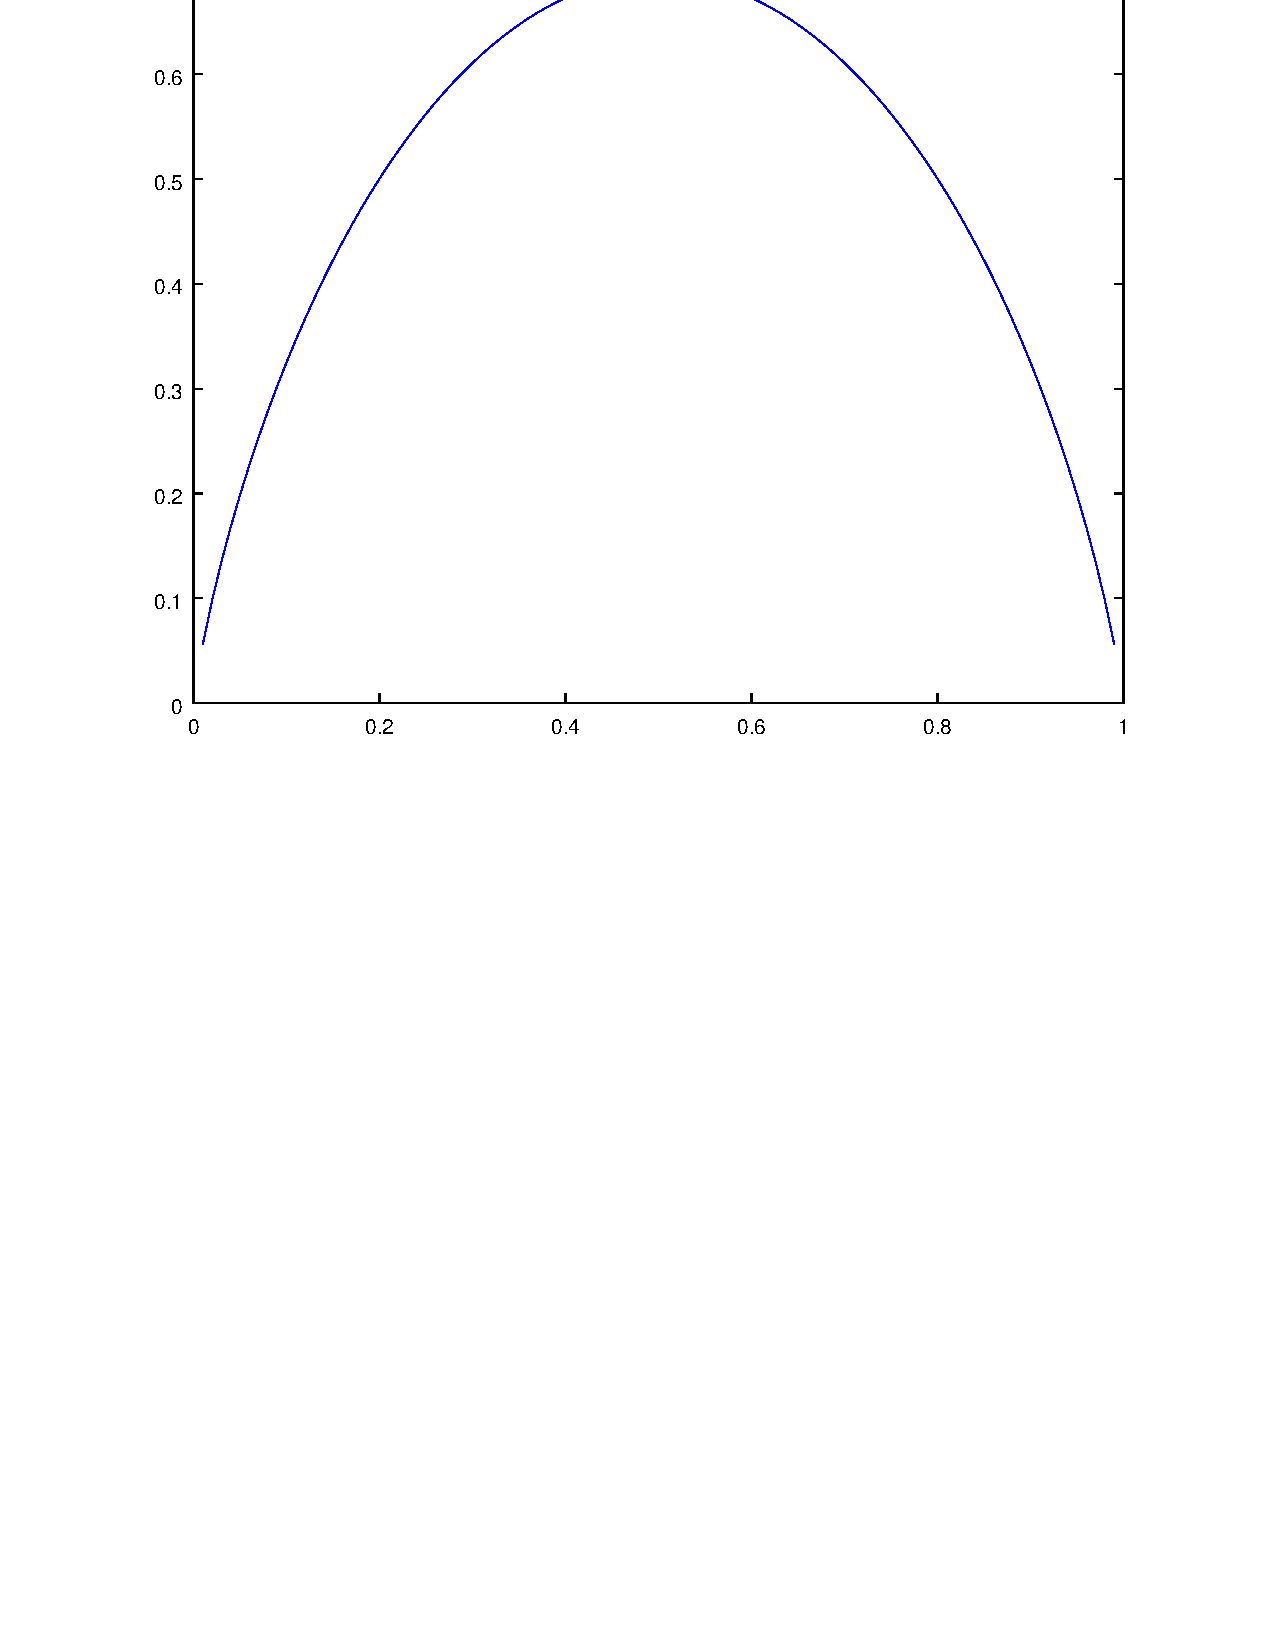
\includegraphics[width=\textwidth]{PlotA2c.pdf}
\end{figure}

\paragraph{d)}
Sei $\mathfrak{M} = (\Omega, \mathcal{F})$ ein Messraum und $\Prob_1$ und $\Prob_2$
zwei Wahscheinlichkeitsmaße auf $\mathfrak{M}$ sowie
$X : \Omega \to \R$ eine endliche Zufallsvariable, d.h.
$\left|X(\Omega)\right| < \infty$.

Zu zeigen ist, dass eine endliche Zufallsvariable mit einer Gleichverteilung
maximale Entropie aufweist. D.h. dass für zwei Wahrscheinlichkeitsmaße $\Prob_1$
und $\Prob_2$ auf $\mathfrak{M}$ mit $\Prob_1(X^{-1}) \equiv c$ gilt
$H_{\Prob_2}^X \le H_{\Prob_1}^X$.

$\Prob_2$ sei gleichverteilt.
\begin{align*}
    H_1^X - H_2^X & = -\sum_{x \in X(\Omega)} \Prob_2(x)\log(\Prob_2(x)) + \sum_{x \in X(\Omega)} \Prob_1(x)\log(\Prob_1(x)) \\
                  & = -|X(\Omega)| \frac{1}{|X(\Omega)|} \log\left(\frac{1}{|X(\Omega)|}\right) + \sum_{x \in X(\Omega)} \Prob_1(x)\log(\Prob_1(x)) \\
                  & = -\log(\frac{1}{|X(\Omega)|}) + \sum_{x \in X(\Omega)} \Prob_1(x)\log(\Prob_1(x)) \\
                  & = -\log(\frac{1}{|X(\Omega)|}) \sum_{x \in X(\Omega)} \Prob_1(x) + \sum_{x \in X(\Omega)} \Prob_1(x)\log(\Prob_1(x)) \\
                  & = -\sum_{x \in X(\Omega)} \Prob_1(x) \log(\Prob_2(x)) + \sum_{x \in X(\Omega)} \Prob_1(x)\log(\Prob_1(x)) \\
                  & = -\sum_{x \in X(\Omega)} \Prob_1(x) \left(\log(\Prob_2(x)) - \log(\Prob_1(x))\right) \\
                  & = -\sum_{x \in X(\Omega)} \Prob_1(x) \log\left(\frac{\Prob_2(x)}{\Prob_1(x)}\right) \\
                  & = D(\Prob_1 || \Prob_2) \ge 0
\end{align*}

Andere Möglichkeit:
Zeige $\log(|X(\Omega)|)$ ist obere Schranke an Entropie für alle $\Prob$ mit
Hilfe der Jensen-Ungleichung und dass $-\log$ konvex ist. Als zweiten Schritt
zeige, dass diese obere Schranke mit einer gleichverteilten ZV angenommen wird.


\end{document}
